\section{Trends in humanoid robotics}

The word ``Robot'' first appeared in Karel Capek's 1921 play \textit{Rossum's Universal Robots} where the \textit{robots} were human-like machines made to replace human workers. It comes from the Czech word ``Robota'' which means ``labour doing compulsory manual works without receiving any remuneration'' or ``to make things manually''. Robots are now very widely used in the manufacturing sector. Robotic technology has been developed and refined so successfully that an entire manufacturing process can be handled by robots alone.

The International standard ISO 3873 defines ``Robot'' as: ``An automatically controlled, reprogrammable, multi-purpose, manipulator, programmable in three or more axes, which may be either fixed in place or mobile for use in industrial automation applications''. This definition restricts the area to only one type of robot, the industrial manipulator. But the inclusion of the perception of the environment and a capacity for action with some level of autonomy the robot leaves the manufacturing plant. The continuous evolution of robots needs a more general definition to include other types of robots in the global robotics area. The Oxford dictionary defines ``Robot'' as ``a machine resembling a human being and able to replicate certain human movements and functions automatically''. Nowadays, the robot is leaving factories and laboratories and slowly entering society in the form of a service robot.

The development of robotics through the ages, makes necessary to do a classification. Based on their ability to make different types of motion, their control architectures differ radically. Five groups of robotic systems can be distinguished by their motion control architecture: industrial, mobile, zoomorphic, anthropomorphic and hybrid robots.

\textit{Industrial robots}. The main characteristic of this group is that all robots are stationary. Industrial robots, including industrial manipulators (Figure \ref{fig:abb}) , are usually designed taking into account different requirements for velocity, load capacity, accessibility, etc. and always have different number of degrees of freedom. These robots are structured to move their end effectors in a determined working environment in one or several systems of coordinates. Although, exceptions may exist when a robot is guided in space (with moving platform) in order to perform a task in another environment. These robots are used when it is necessary to attend rather extensive but permanent working zones, working mainly with different types of objects and environments and does not exist human-robot interaction.
\begin{figure}[!hbt]
\centering
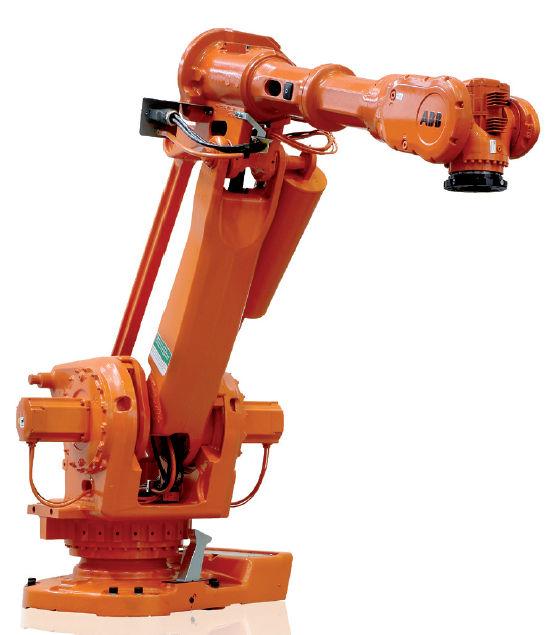
\includegraphics[scale=0.35]{abb.jpg}
\caption{ABB industrial manipulator}
\label{fig:abb}
\end{figure}
 
\textit{Mobile robots}. This group has more motion capacity due to implemented wheel based platform systems (Figure \ref{fig:mobile}). They can execute different telecontrolled tasks or are driven by the environmental information received from the integrated sensorial system. The motorized turtle designed in 1948 by Walter was the first predecessor. From the beginning of the sixties mobile robots were designed and implemented within industry. These robots were able to transport parts from one point of the production line to another, guided by preplanned paths materialized by the electromagnetic or photoelectric bands from circuits mounted into the floor. From the beginning of the seventies a lot of work was related to major autonomy of mobile robots. It involved providing the mobile robot with a vision system \textcolor{red}{[Moravec, 1981]}. Finally, from the beginning of the eighties, when more complex and precise sensorial systems appeared, the development of architectures for control of mobile robots was concentrated on the superficial intelligence and decision making systems \textcolor{red}{[Bares, 1998], [Thorpe, 1990]}. Mobile robots provided with this kind of control system are usually able to plan motions and avoid obstacles. Today, research is also centred on human-mobile robot interaction \textcolor{red}{[Khamis 2007]}. 

\begin{figure}[!hbt]
\centering
\subfigure[TurtleBot mobile robot]{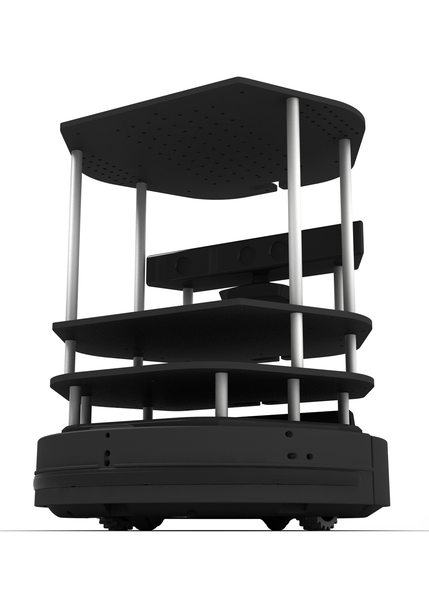
\includegraphics[width=30mm]{turtlebot.png}}\hspace{10mm}
\subfigure[MAGGIE social robot from UC3M]{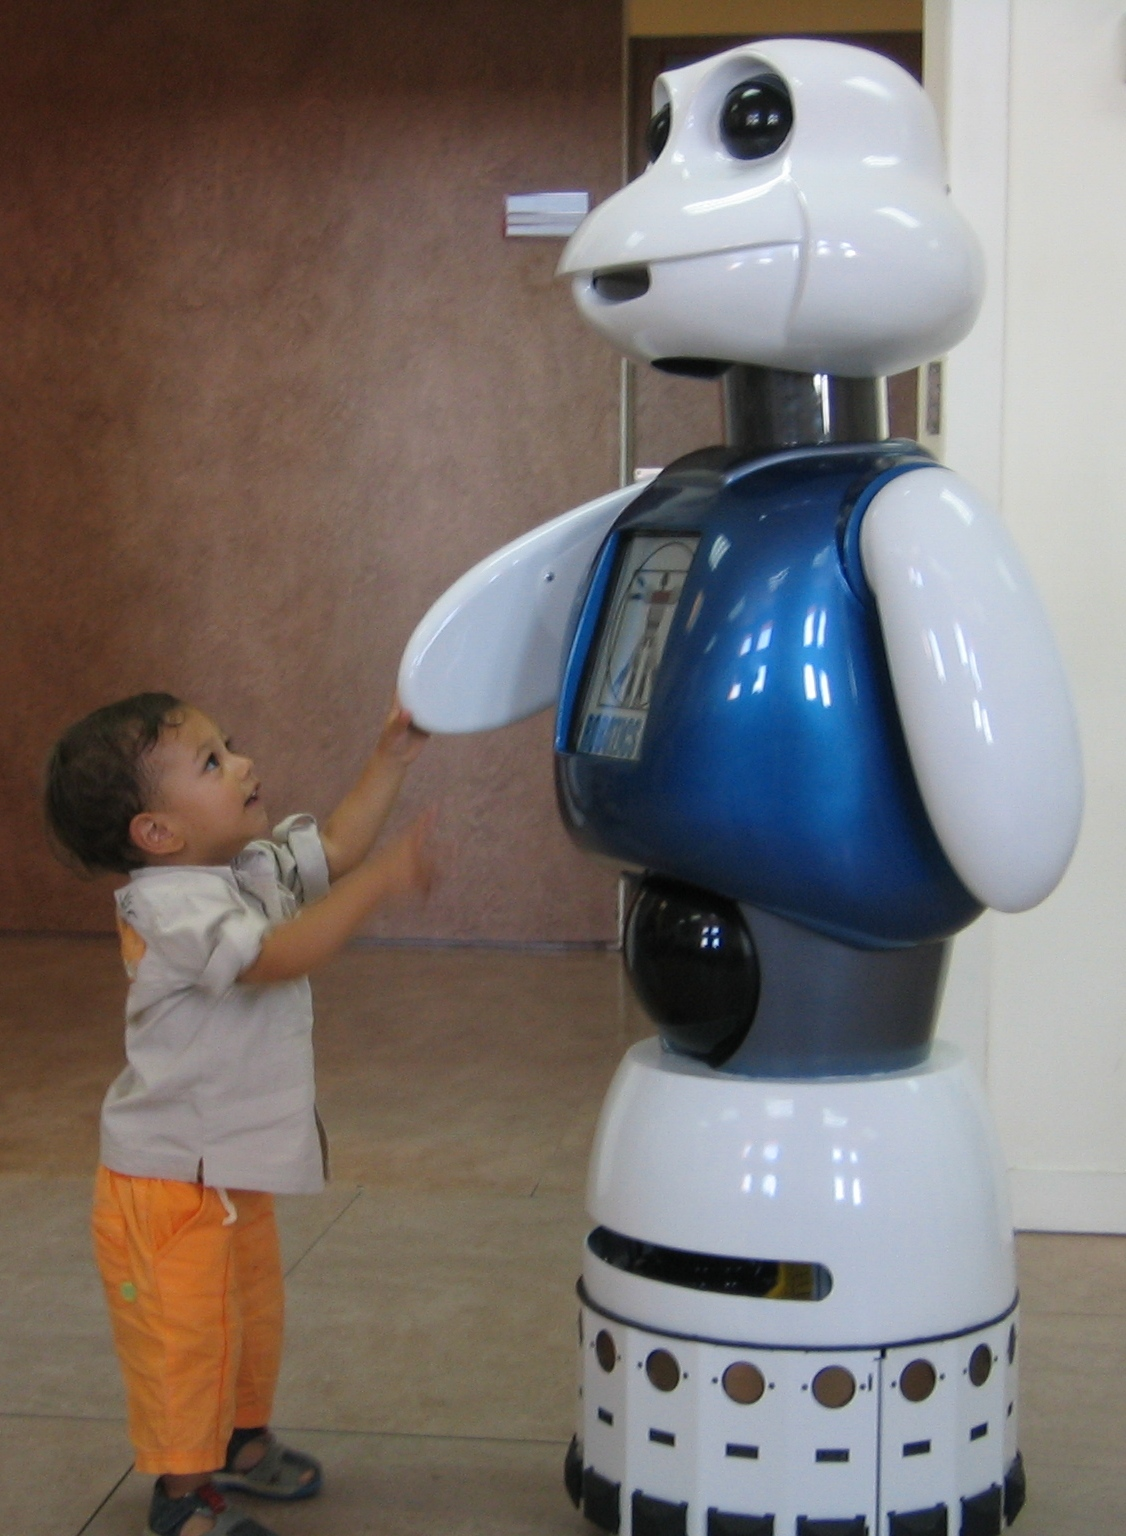
\includegraphics[width=30mm]{maggie.jpg}}
\caption{Mobile robots}
\label{fig:mobile}
\end{figure}

\textit{Zoomorphic robots}. This type of robot is characterized by the locomotion system which imitates the locomotion of diverse living beings. Although there can be a lot of morphological differences between all variations of zoomorphic systems, it is possible to distinguish two basic categories: walking and non-walking zoomorphic architectures. An example of non-walking zoomorphic robot is the modular snake-like robot in Figure \ref{fig:zoo} (a). Walking zoomorphic robots are developed to work in every king of terrain and they have a really wide range of applications. It could be spatial research, out-of-the-way terrain exploration, or volcanic research. Animal-like robots try to imitate the movements of animals and are usually constructed for research and entertainment. The control of this kind of robot is more complicated than control of a mobile or polyarticulated robot because of the need to maintain the equilibrium at every stage of motion. Figure \ref{fig:zoo} (b) shows the WildCat walking zoomorphic robot developed by Boston Dynamics.

\begin{figure}[!hbt]
\centering 
\subfigure[Non-walking zoomorphic robot]{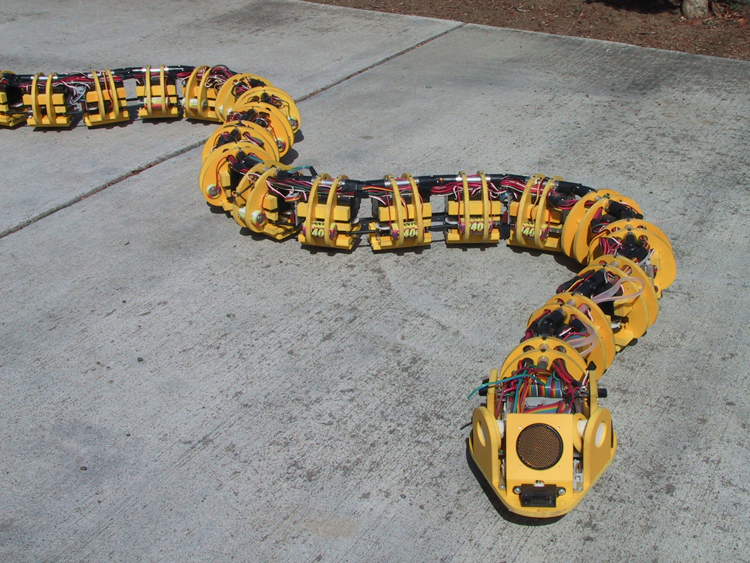
\includegraphics[width=40mm]{snake.jpg}}\hspace{10mm}
\subfigure[WildCat walking zoomporphic robot]{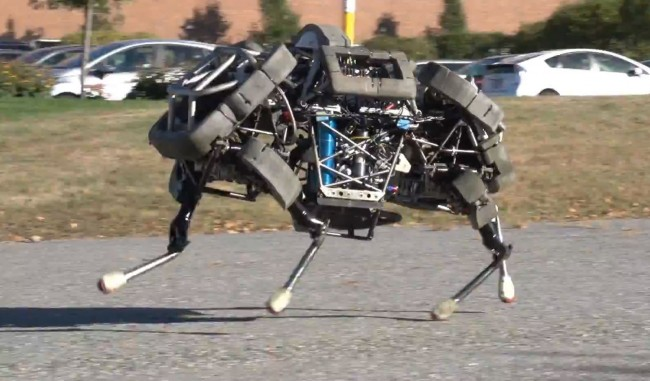
\includegraphics[width=40mm]{wildcat.jpg}}
\caption{Zoomporphic robots}
\label{fig:zoo}
\end{figure}

\textit{Anthropomorphic robots (Androids)} or humanoid (bipedal) robots. These robots try to reproduce the body and behaviours of a human being. Presently the research on humanoids is increasing rapidly, although, there still remains a lot of work ahead. One of the basic challenges in this field is to reproduce human-like motion abilities beginning with the bipedal locomotion \textcolor{red}{[Hirai 98]}. The motion control architecture in this case is the most complex compared with the other robot types presented above. The main challenge is being able to control and coordinate in real time the dynamics of the entire body and maintain the equilibrium in the single support phase, i.e. when the robot is supported only by one foot. The control architecture of this kind of robot is an aim of the presented research and will be discussed and developed further in the following chapters. Figure \ref{fig:humanoid} shows two examples of humanoid robots: (a) is Asimo Robot developed by Honda and (b) is TEO robot from UC3M.

\begin{figure}[!hbt]
\centering 
\subfigure[ASIMO robot]{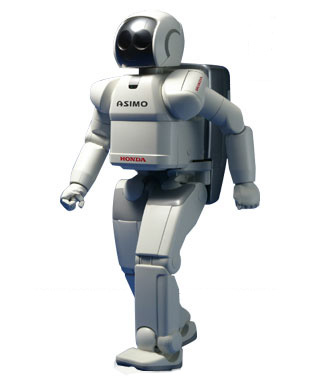
\includegraphics[width=30mm]{asimo.jpg}}\hspace{10mm}
\subfigure[TEO robot]{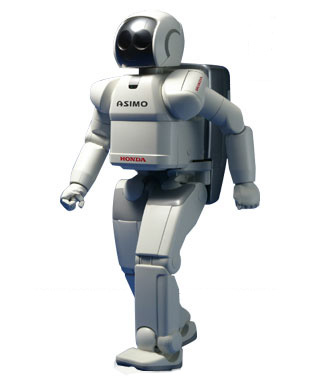
\includegraphics[width=30mm]{asimo.jpg}}
\caption{Humanoid robots}
\label{fig:zoo}
\end{figure}


Another complex aspect related to androids is the ability to reproduce the human upper body, especially the face. The difference between a humanoid robot and android is only skin-deep. The latter looks exactly like a human on the outside, but internally has the mechanics of a humanoid robot. But the human-like appearance can be controversial. In 1970, Masahiro Mori presented his hypothesis about the \textit{Uncanny Valley} (Figure \ref{fig:valley}). Mori's insight was that people would react with revulsion to human-like robots, whose appearance resembled, but did not quite replicate, that of a real human. The Uncanny Valley has become more relevant in the past few years since robots that actually look and move like humans are starting to become a reality. In fact, researchers currently debate over whether they should try to overcome the uncanny valley or simply design robots that are more mechanical in appearance.

\begin{figure}[!hbt]
\centering
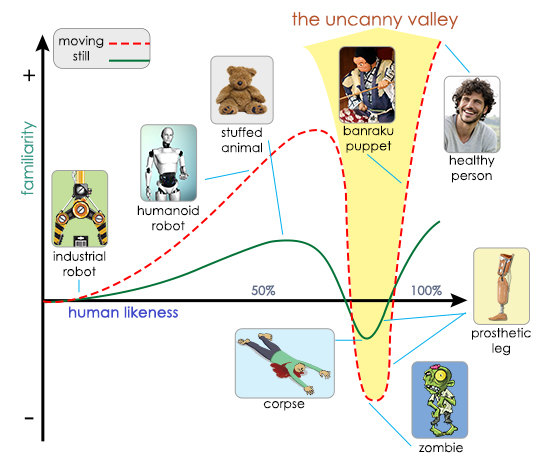
\includegraphics[scale=0.45]{valley.jpg}
\caption{Uncanny valley}
\label{fig:valley}
\end{figure}


\textit{Hybrid robots.} These type  of robots combine properties of various types of other robots. Usually they are a combination of a wheelbase (mobile robot) with an anthropomorphic body. Some examples are Justin robot from the German Aerospace Center (DLR) and TIAGO robot from PAL Robotics (Figure \ref{fig:hybrid}). They are both mainly involved in manipulation tasks (grasping, picking and placing, etc.) and the problem of locomotion in not considered as in humanoids. 

\begin{figure}[!hbt]
\centering 
\subfigure[Justin robot]{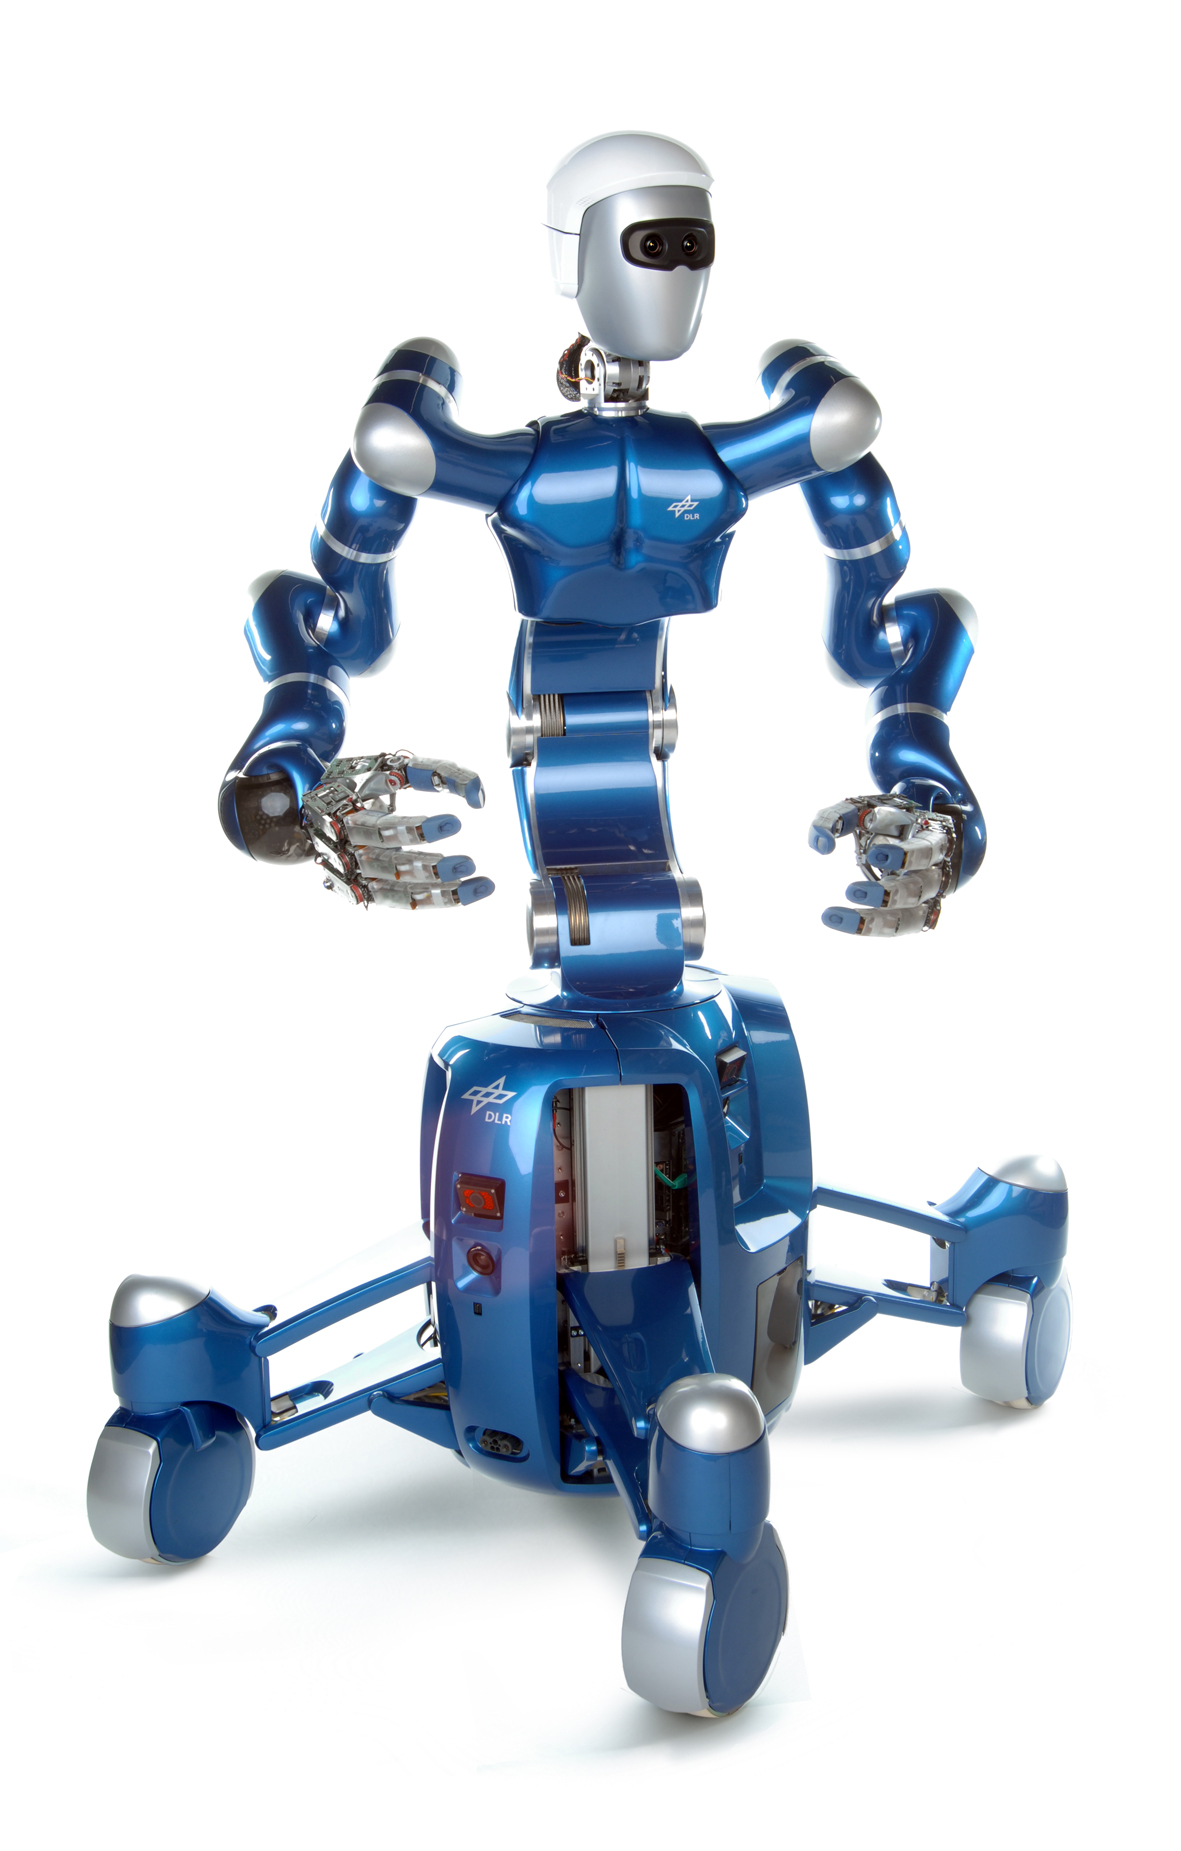
\includegraphics[width=30mm]{justin.jpg}}\hspace{10mm}
\subfigure[TIAGO robot]{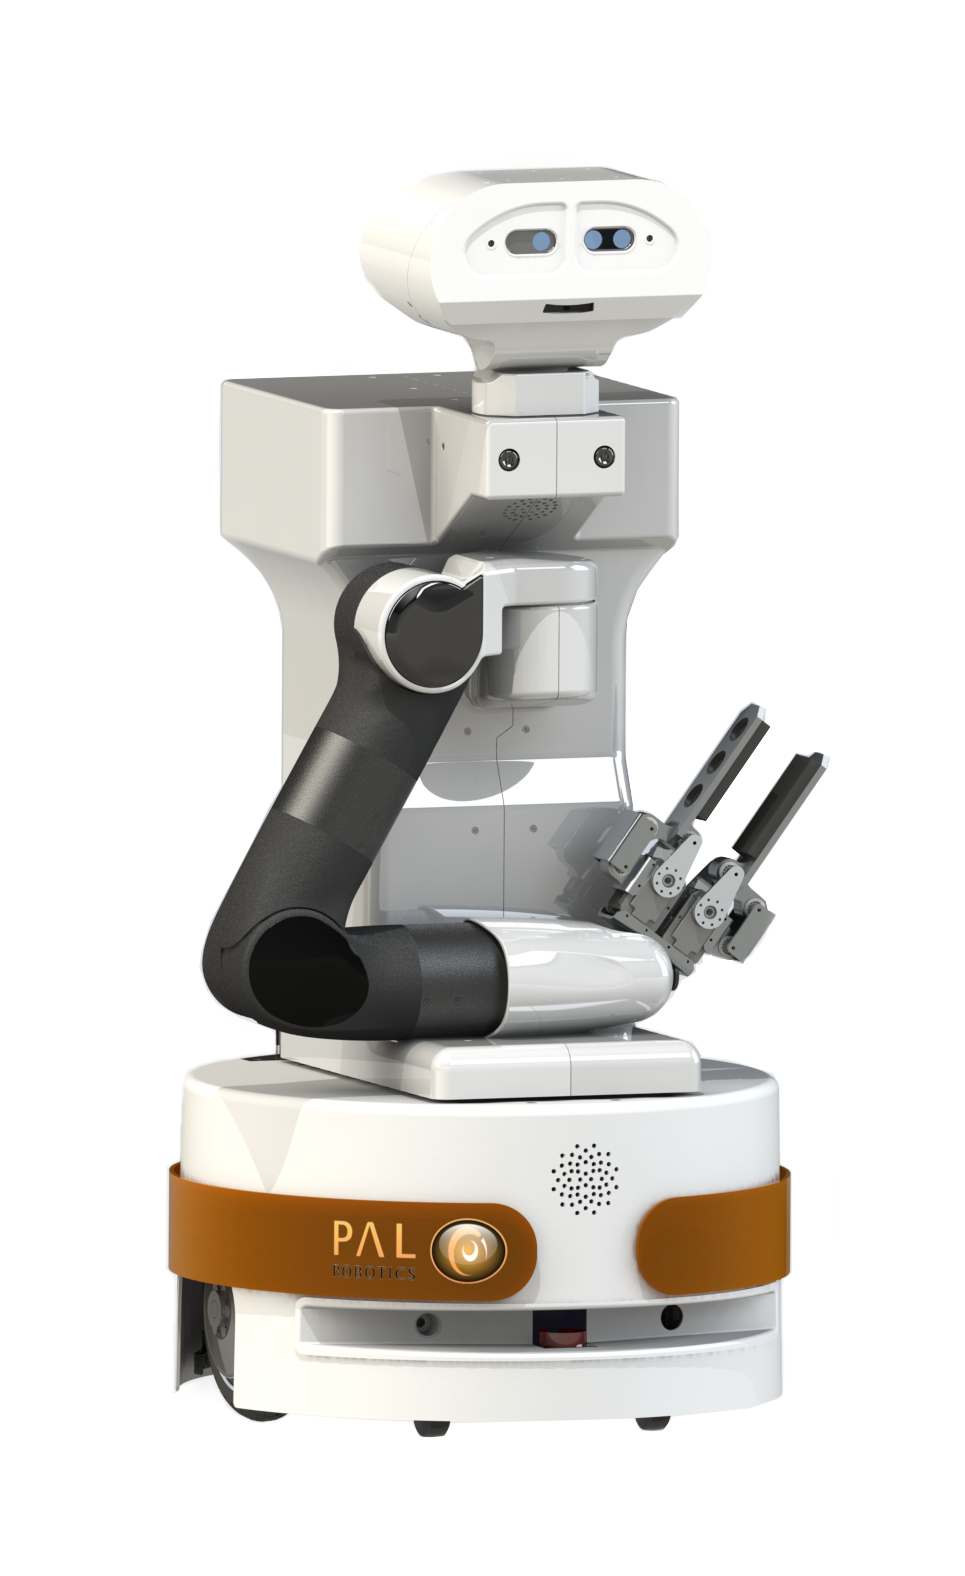
\includegraphics[width=30mm]{tiago.jpg}}
\caption{Hybrid robots}
\label{fig:hybrid}
\end{figure}

\newpage












